
\documentclass[11pt,a4paper,oneside]{article}
\usepackage[T1]{fontenc} 
\usepackage[utf8]{inputenc}
\usepackage[main=english]{babel}
\usepackage{graphicx} % 1pt = 0.035146cm
\usepackage[justification=default]{subfig} %Manage sub-figures 
\usepackage[update]{epstopdf}
\usepackage[labelfont=bf]{caption}
\usepackage{titlesec} % Allows customization of titles
\usepackage{booktabs}
\usepackage{gensymb}
\usepackage{color}
\usepackage[textwidth = 460pt,top = 80pt, bottom = 60pt]{geometry}
\usepackage{soul}
\newcommand{\hlc}[2][yellow]{{\sethlcolor{#1}\hl{#2}}}
\usepackage[inline]{enumitem}
\usepackage[symbol]{footmisc}

\renewcommand{\thefootnote}{\fnsymbol{footnote}}

%--------------------------------------------------------------------------------
%       MATH PACKAGES
%--------------------------------------------------------------------------------
\usepackage{amsmath}
%\usepackage{mathtools}
\usepackage[leqno,fleqn,intlimits]{empheq}
\usepackage{bm}
%\usepackage{amssymb}
\usepackage{empheq}
\usepackage[inline]{enumitem}
%--------------------------------------------------------------------------------
%       MATLAB CODE
%--------------------------------------------------------------------------------
\usepackage{mcode}
%--------------------------------------------------------------------------------
%       MY COMMANDS
%--------------------------------------------------------------------------------
\renewcommand{\vec}[1]{\mathbf{#1}}
\newcommand{\tr}{\textcolor{red}}
\newcommand{\mathbi}[1]{\bm{\textbf{\em #1}}}
%--------------------------------------------------------------------------------
%       BIBLIOGRAPHY PACKAGES
%--------------------------------------------------------------------------------
% \usepackage{csquotes}
% \usepackage[sorting=nyt,%
% sortcites=true,%
% bibencoding=ascii,%
% autopunct=true,%
% hyperref=true,%
% language=auto,%
% %backref=true,%
% url=false,%
% maxcitenames=10,%
% minbibnames = 3,%
% maxbibnames=3,%
% giveninits, 
% natbib = false,
% isbn=false,%
% backend=biber]{biblatex}
% \addbibresource{bibliograhy_assignment.tex}
%--------------------------------------------------------------------------------
%       MISCELLANEA
%--------------------------------------------------------------------------------
\usepackage[]{hyperref}
\usepackage{cleveref}
%%% CREF setup
\crefname{equation}{Eq.}{Eqs.}
\crefname{table}{Table}{Tables}
\crefname{figure}{Fig.}{Figs.}

%--------------------------------------------------------------------------------
%       TITLE SECTION
%--------------------------------------------------------------------------------
\newcommand\headlinecolor{\normalcolor}

\makeatletter
\renewcommand*\maketitle{%
    \begingroup
    \centering
    \fontsize{15}{15}% 72pt on 80pt leading
    \selectfont
    \headlinecolor
    \@title\\
    \vspace{5mm}
    \@author
    \par
    \vskip1in
    \endgroup
    \vspace{-22mm}
}
\makeatother


\title{MSAS -- Assignment \#2: Modeling} % Article title
\author{\large Lorenzo Cucchi, 221732}
\date{}

%--------------------------------------------------------------------------------
% HEADING packages
\usepackage{fancyhdr} % Headers and footers control
\setlength{\headheight}{15.2pt}
\pagestyle{fancyplain} % Defines a new header for all pages (absolutely all pages, use fancy to exclude title-page and chapters, if book class is used) 
\fancyhf{} % clears the header and footer, otherwise the elements of the default "plain" page style will appear
%
\lhead{Lorenzo Cucchi, MSAS -- Assignment \#2}
\rhead{\vspace{-0.5cm}
\includegraphics[width=0.3\textwidth]{gfx/newlogo.eps}}
\lfoot{AY 2023-24 -- Prof.\ F.\ Topputo; TA: C.\ Balossi, S.\ Borgia}
\rfoot{\thepage}
%--------------------------------------------------------------------------------
%       BEGIN DOCUMENT
%--------------------------------------------------------------------------------
\begin{document}

\maketitle

\thispagestyle{fancy}
%--------------------------------------------------------------------------------
%       MODELING PARADIGMS, BASIC SYSTEMS
%--------------------------------------------------------------------------------


\section*{Exercise 1}
The rocket engine in Figure \ref{fig:therm} is fired in laboratory conditions. With reference to Figure \ref{fig:therm}, the nozzle is made up of an inner lining ($k_1$), an inner layer having specific heat $c_2$ and high conductivity $k_2$, an insulating layer having specific heat $c_4$ and low conductivity $k_4$, and an outer coating ($k_5$). The interface between the conductor and the insulator layers has thermal conductivity $k_3$.

\subsection*{1.1) Part 1: Parameters definition}
Select the materials of which the nozzle is made of\footnote{The interface layer is not made of a physically existing material, though it produces a thermal resistance. For this layer, the value of the thermal resistance $R_3$ can be direcly assumed, so avoiding to choose $k_3$ and $\ell_3$.}, and therefore determine the values of $k_i$ ($i=1,\dots,5$), $c_2$, and $c_4$. Assign also the values of $\ell_i$ (i=1,\dots,5), $L$, and $A$ in Figure \ref{fig:therm}.
\begin{figure}[h!]
\centering
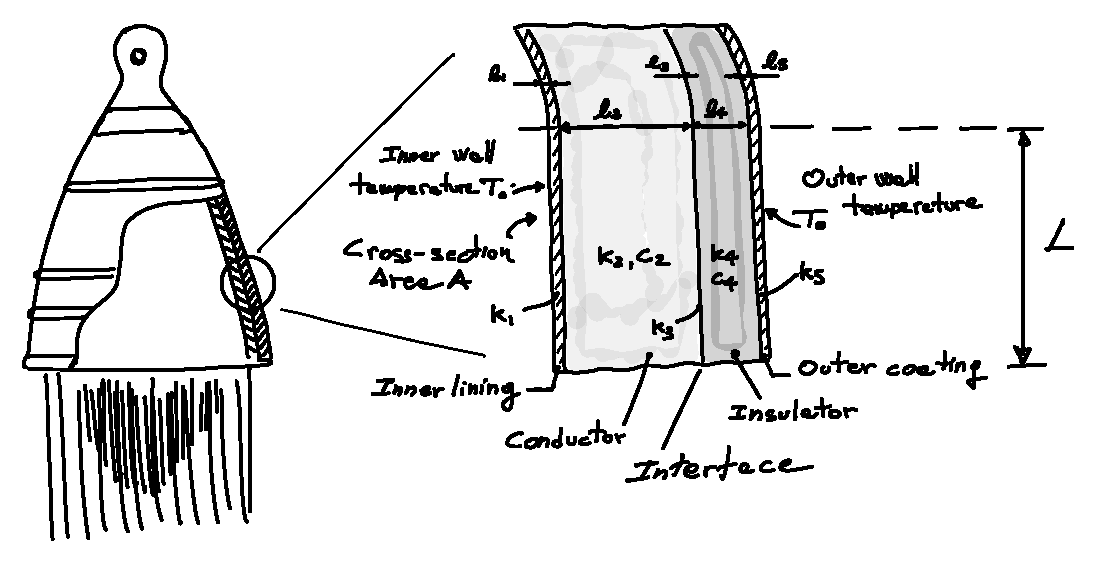
\includegraphics[width=0.8\textwidth]{gfx/fig_therm.pdf}
\caption{\label{fig:therm} Real thermal system.}
\end{figure}

\subsection*{1.2) Part 2: Causal modeling}
Derive a physical model and the associated mathematical model using one node per each of the five layers and considering that only the conductor and insulator layers have thermal capacitance. The inner wall temperature, $T_i$, as well as the outer wall temperature, $T_o$, are assigned.
Using the mathematical model, carry out a dynamic simulation \underline{in MATLAB} to show the temperature profiles across the different sections. At initial time, $T_i(t_0)=T_o(t) = 20\ {\rm C^\circ}$. When the rocket is fired, $T_i(t) = 1000\ {\rm C^\circ}$, $t\in[t_1,\,t_f]$, following a ramp profile in $[t_0,\,t_1]$. Integrate the system using $t_1 = 1\ {\rm s}$ and $t_f = 60\ {\rm s}$.

\subsection*{1.3) Part 3: Acausal modeling}
a) Reproduce \underline{in Simscape} the physical model derived in Part 2. Run the simulation from $t_0 = 0\ {\rm s}$ to $t_f = 60\ {\rm s}$ and show the temperature profiles across the different sections. Compare the results with the ones obtained in point 1.2). 
b) Which solver would you choose? Justify the selection based on the knowledge acquired from the first part of the course.
c) Repeat the simulation in Simscape implementing two nodes for the conductor and insulator layers and show the temperature profiles across the different sections.
\medskip

\medskip \hrule \medskip
\rightline{\small(15 points)}

The selection of the layers materials has grate effect on the thermal behavior of the system. 
In particular, the thermal conductivity of the materials is the main parameter that affects 
the heat transfer between the layers. The thermal conductivity of the materials can be found 
in literature, the choiche of the material is based on the design requirements assigned. 
The chosen materials are reported in \autoref{tab:materials}.


\begin{table}[h!]
    \centering
    \begin{tabular}{ |c|c|c|c|c|c| }
        \hline
    \textbf{Layer} & \textbf{Material} & \textbf{k} $[W/(mK)]$& \textbf{c} $[J/(KgK)]$& $\mathbf{\rho}$ $[kg/m^3]$ & \textbf{th} [mm] \\
    \hline\hline
    Inner lining & Carbon-Phenolic comp. & 1.5 & $-$ & 1650 & 4\\ \hline
    Conductor & Graphite G-348 & 130 & 750 & 1830 & 10\\  \hline
    Insulator & Cork & 0.07 & 2100 & 485 & 8\\ \hline
    Outer coating & Alluminium 6061T6 & 160 & $-$ & 2700 & 2\\ \hline  
    \end{tabular}\caption{Materials properties}\label{tab:materials}
\end{table}

The carbo-phenolic composite is used as inner lining because of its low thermal conductivity and 
its high thermal resistance, the inner lining is in direct contact with the conductor. Graphite has
been chose as the conductor because of its good thermal conductivity and low density compared to metals,
moreover its mechanical characteristics don't vary with temperature. The interface between the conductor
and the insulator is modelled as a layer with thermal conductivity obtained from literature and derived
from the contact resistance $R_\theta =th/(Ak)$ which is approximately $R_\theta = 7\times 10^{-3} [m^2K/W]$.
Not considering an interface cause the temperature to be almost equal at the interface.\
The insulator is made of cork which has a low thermal conductivity and low density and is in contact 
with alluminium which act as the outer coating.\

The nozzle is modelled as a flat plate, to do this we have to define an exchange area $A=1\ [m^2]$ 
and a length $L=0.5 [m]$ derived from a nozzle with a $D_{exit}=0.636\ [m]$. 

\begin{figure}[h!]
    \centering
    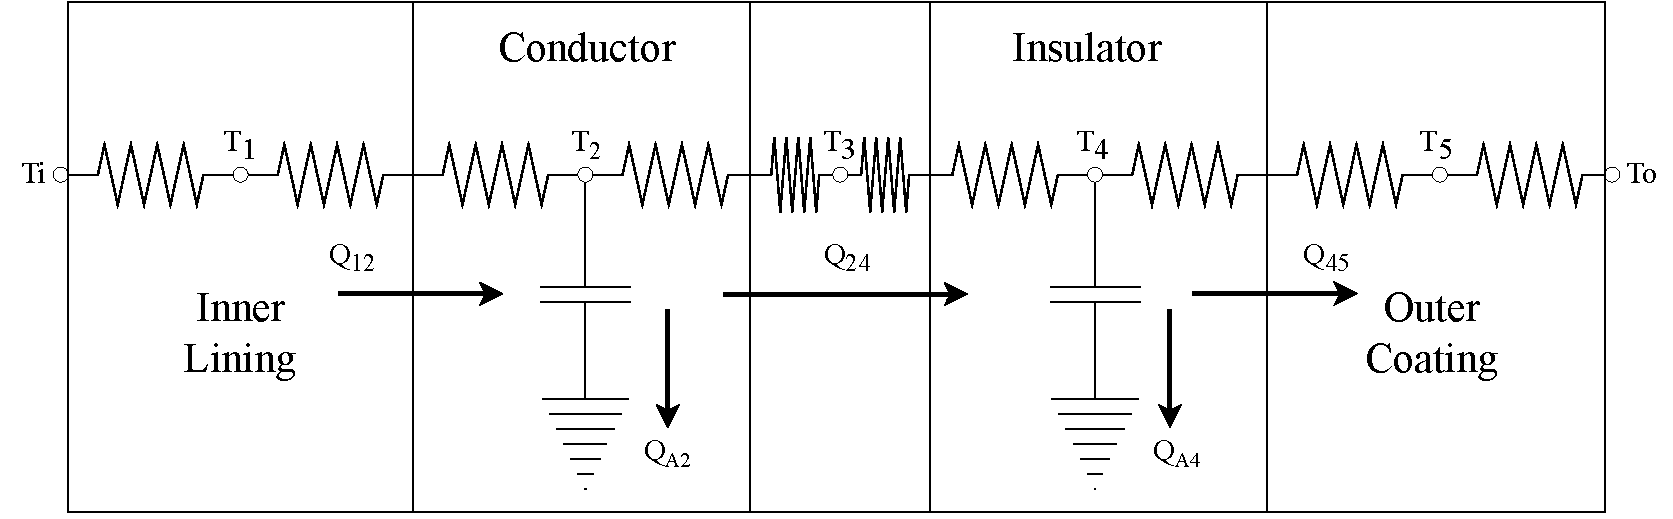
\includegraphics[width=1\textwidth]{gfx/thermal_model.pdf}
    \caption{\label{fig:thermal} Physical model of the system.}
\end{figure}
    
The physical model that approximantes the system uses only one node per layer and it's represented in 
\autoref{fig:thermal}. The thermal capacitance is modelled as a thermal mass $C_i=c_i\rho_i V_i$
the thermal resistance is modelled as $R_i=th_i/(k_iA_i)$, every resistance in \autoref{fig:thermal}
is actually divided in half for every layer. Using this definitions it's possible to derive the 
mathematical model represented from the following equations:

\begin{equation}
    \begin{cases}
      Q_{A2}=Q_{12}-Q_{24}\\
      Q_{A4}=Q_{24}-Q_{45}
    \end{cases}\
    \Rightarrow\
    \begin{cases}
        C_{2}\frac{dT_2}{dt}=\frac{T_i-T_2}{R_1+R_2/2} - \frac{T_2-T_4}{R_2/2+R_3+R_4/2}\\
        C_{4}\frac{dT_4}{dt}=\frac{T_2-T_4}{R_2/2+R_3+R_4/2} - \frac{T_4-T_o}{R_4/2+R_5}\\
    \end{cases}
\end{equation}

This set of equations can be transformed in a state space model:
\begin{equation}
    \vec{\dot x}=\vec{A}\vec{x}+\vec{B}\vec{u} \ , \ \ \vec{x}=\begin{bmatrix} T_2 \\ T_4 \end{bmatrix} \ , \ \ \vec{u}=\begin{bmatrix} T_i \\ T_o \end{bmatrix}
\end{equation}

\begin{equation}
    \vec{A} = 
    \begin{bmatrix}
        -\frac{R_1+R_2+R_3+R_4/2}{C_2(R_1+R_2/2)(R_2/2+R_3+R_4/2)} & \frac{1}{C_2(R_2/2+R_3+R_4/2)}\\
        \\
        \frac{1}{C_4(R_2/2+R_3+R_4/2)} & -\frac{R_2/2+R_3+R_4+R_5}{C_4(R_2/2+R_3+R_4/2)(R_4/2+R_5)}
    \end{bmatrix}
\end{equation}

\begin{equation}
    \vec{B} = 
    \begin{bmatrix}
        \frac{1}{C_2(R_1+R_2/2)} & 0\\
        \\
        0 & \frac{1}{C_4(R_4/2+R_5)}
    \end{bmatrix}
\end{equation}
It's possible to integrate the system using the \textbf{ode45} solver in MATLAB, since the eigenvalues of the state 
matrix $\vec{A}$ are $\lambda \approx [-0.029,-0.004]$. After the integration the temperature histories
of all nodes are retrieved performing an heat balance of the system and are displayed in \autoref{fig:ex1-1}.

\begin{figure}[h]
    \centering
        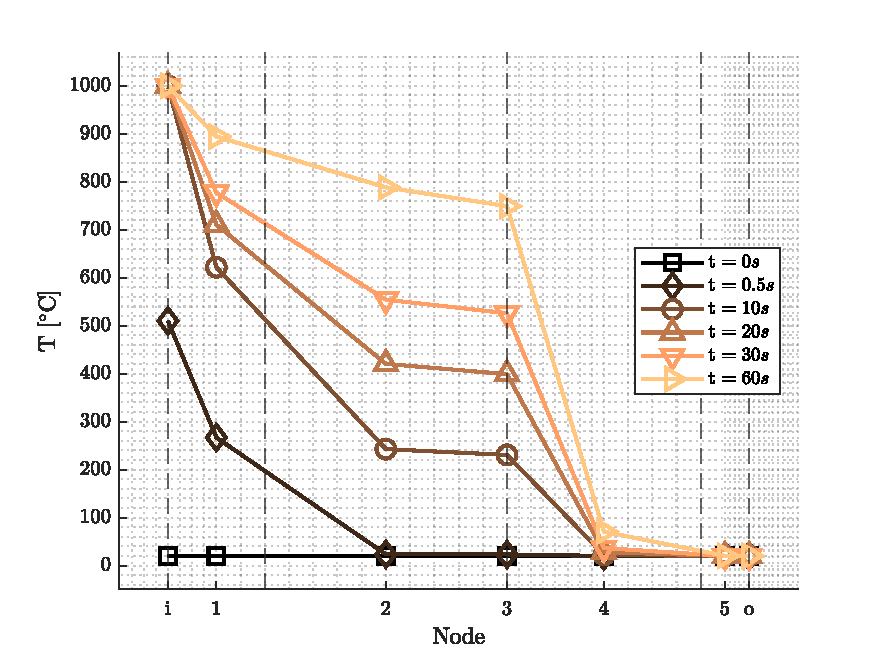
\includegraphics[width = 0.9\textwidth]{gfx/ex1-1.pdf}
        \caption{Evolution of temperature in single node casual model.}\label{fig:ex1-1}
\end{figure}

The acausal model is implemented in Simscape using the thermal library, the temperature source is defined
with a ramp block and a saturation one and is connected to a controlled temperature source block. The temperature
source also receive in input the ambient temperature which is $20^{\circ}C$, the temperature source is connected to
the inner wall surface of the nozzle. The outer wall surface is connected to the ambient temperature block.\
To model the inner and outer layers two conductive heat transfer blocks are used for each, the conductive 
and insulator layers are modelled with a single thermal mass and two conductive heat transfer blocks. 
The interface layer is modelled with two thermal resistances, this blocks are used since from literature it was
possible to obtain only a thermal surface resistance and the layer has no thickness.\

The simulation is run from $t_0=0\ [s]$ to $t_f=60\ [s]$ and the temperature histories are displayed in \autoref{fig:ex1-2}.

\begin{figure}[h!]
    \centering
        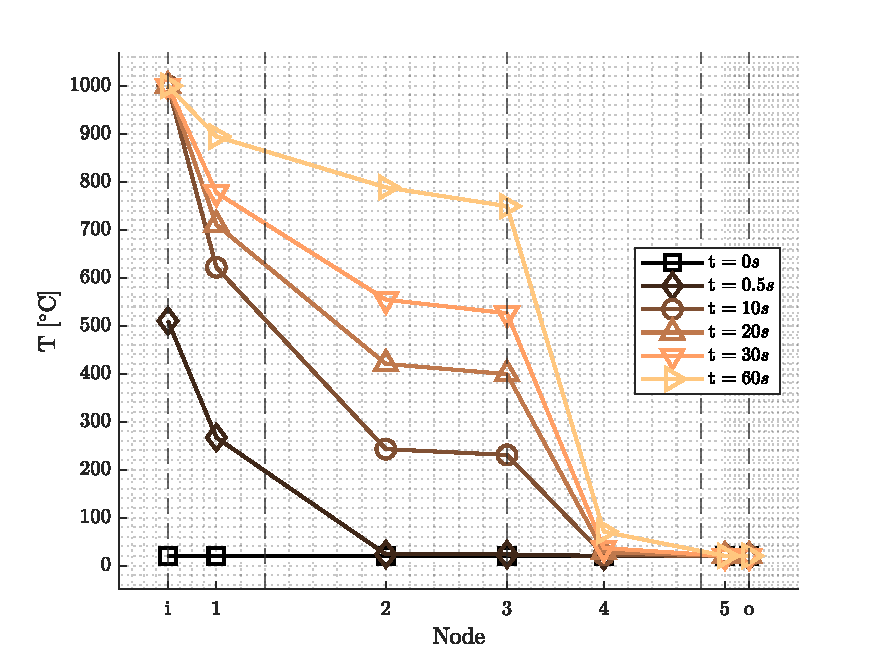
\includegraphics[width = 0.75\textwidth]{gfx/ex1-2.pdf}
        \caption{Evolution of temperature in single node acasual model.}\label{fig:ex1-2}
\end{figure}

\begin{figure}[h!]
    \centering
        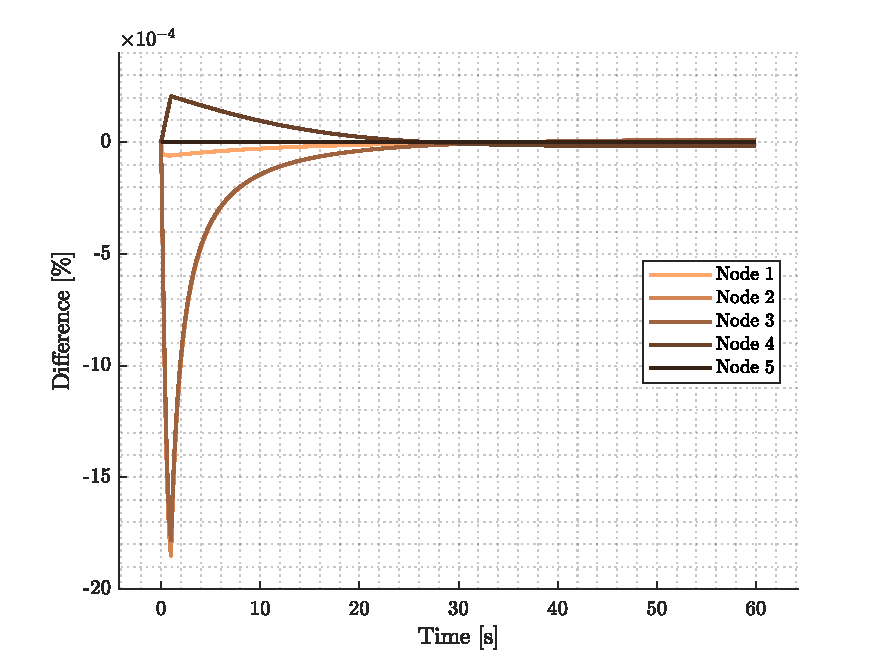
\includegraphics[width = 0.75\textwidth]{gfx/ex1-5.pdf}
        \caption{Percentual difference between casual and acasual model.}\label{fig:ex1-5}
\end{figure}

The solver used is the Simscape \textbf{Trapezoidal Rule} local solver with a fixed time step of $0.1\ [s]$, the solver is chosen
since it's A-stable and can handle stiff systems. The simulation results are almost identical to the ones
obtained with the \textbf{ode45} solver for the casual model, the difference is neglectable and it's shown in 
\autoref{fig:ex1-5}, node 2 and 3 differences from the casual model are almost identical in the model. 
Another viable solver is the \textbf(ode23t) which is also a trapezoidal rule solver but has variable-time stepping,
the result would be more precise near the temperature source step but it wouldn't provide more benefits after the
temperature source is stable. The fixed time step is useful in case of real time simulation interfaced
with control systems. 
It's possible to add multiple nodes to the simulation by splitting the thermal mass and the thermal resistance 
following the position of the additional nodes. In this case the conductor and the insulator will have an additional node each,
for both three thermal conductive heat transfer blocks are used each with a third of the layer thickness, 
the thermal mass is divided in two identical parts. The simulation is run from $t_0=0\ [s]$ to $t_f=60\ [s]$ 
and the temperature history of the nozzle is displayed in \autoref{fig:ex1-3} and in \autoref{fig:ex1-4} the 
temperature history of each node is shown.

\begin{figure}[h!]
    \centering
        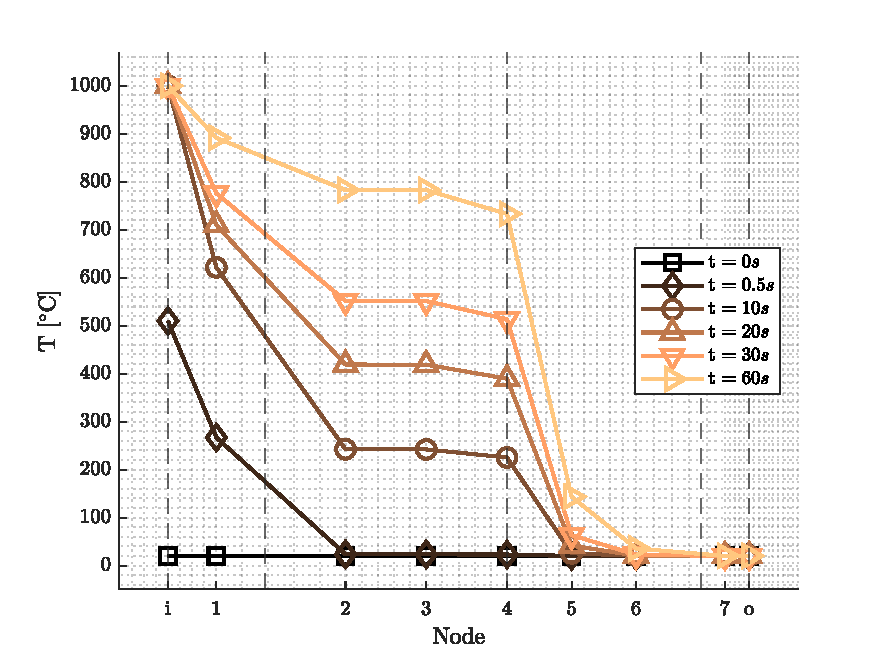
\includegraphics[width = 0.7\textwidth]{gfx/ex1-3.pdf}
        \caption{Percentual difference between casual and acasual model.}\label{fig:ex1-3}
\end{figure}

\begin{figure}[h!]
    \centering
        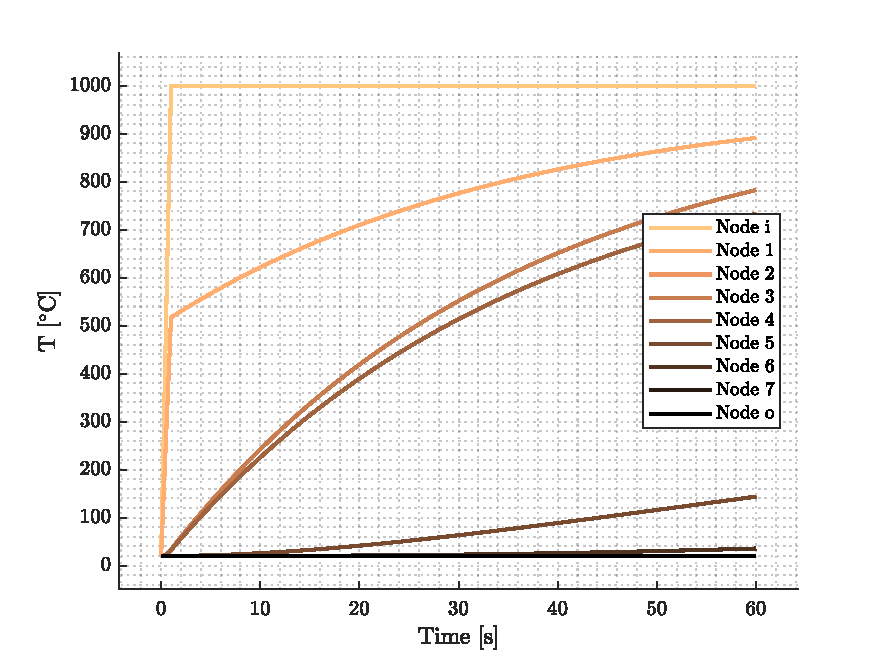
\includegraphics[width = 0.7\textwidth]{gfx/ex1-4.pdf}
        \caption{Percentual difference between casual and acasual model.}\label{fig:ex1-4}
\end{figure}


\clearpage
\section*{Exercise 2}
The real system of an electric propeller engine is depicted in Figure \ref{fig:propeller}. It is composed by a DC permanent magnet motor which drives a propeller shaft. Between the motor and propeller shaft there is a single stage gear box to regulate the angular speed ratio. Moreover, to avoid overheating of the gear unit, the system is augmented by a cooling system where a fluid exchanges heat with the gear box itself. In Figure \ref{fig:blocks scheme} a functional breakdown structure of the system is shown. 



\begin{figure}[h!]
\centering
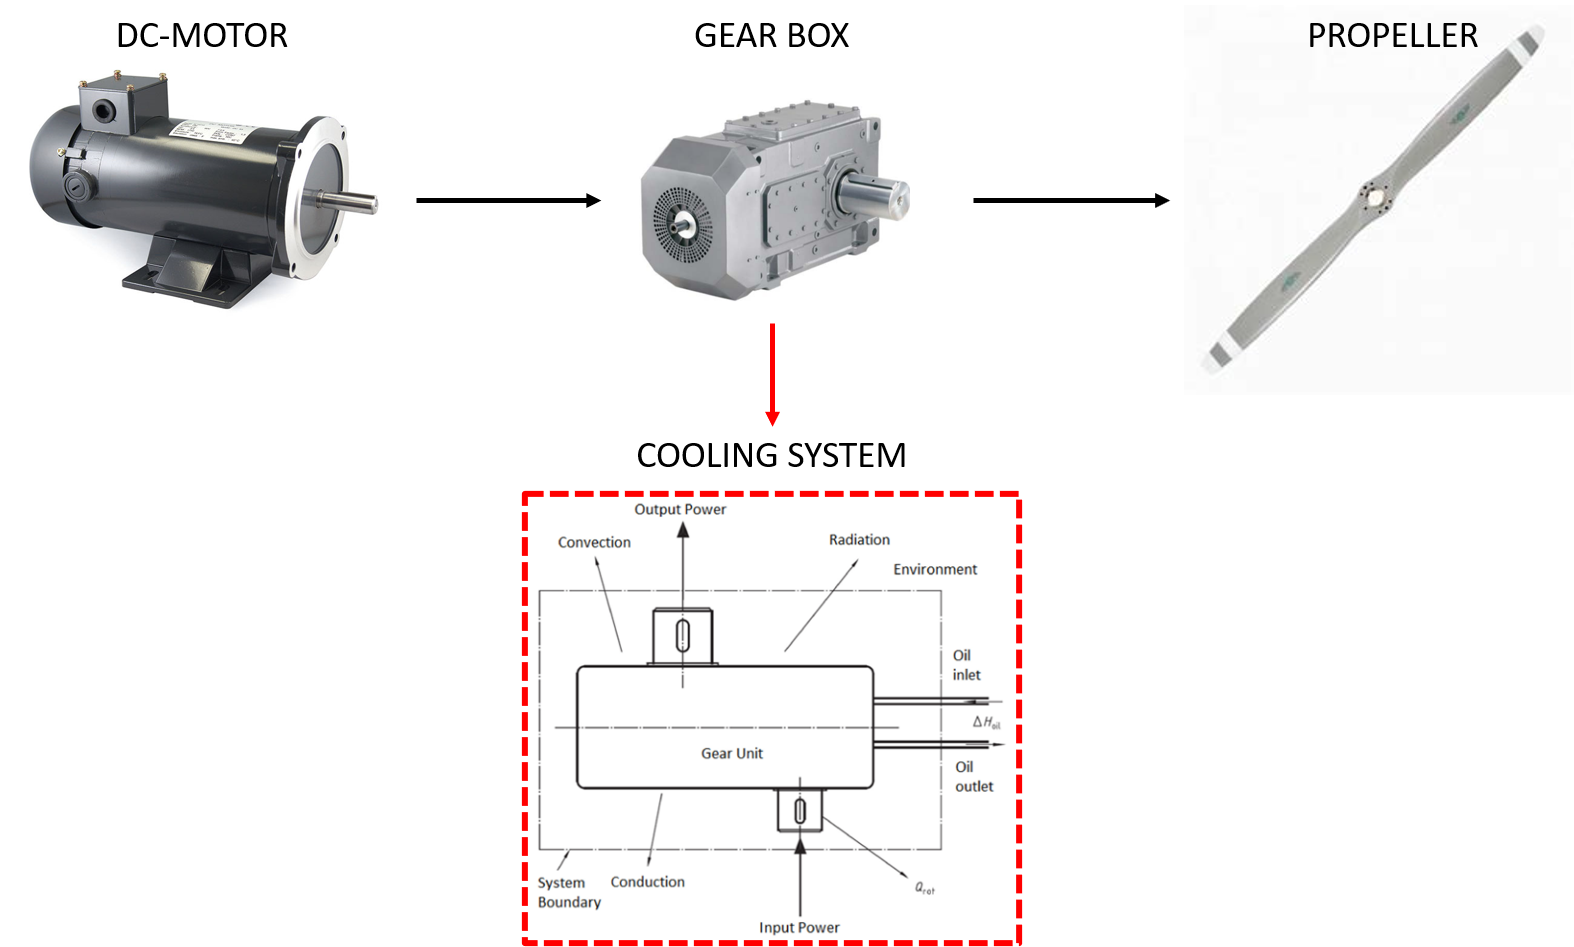
\includegraphics[width=0.8\textwidth]{gfx/RealSystem_msas.png}
\caption{\label{fig:propeller} Real system.}
\end{figure}


\begin{figure}[h!]
\centering
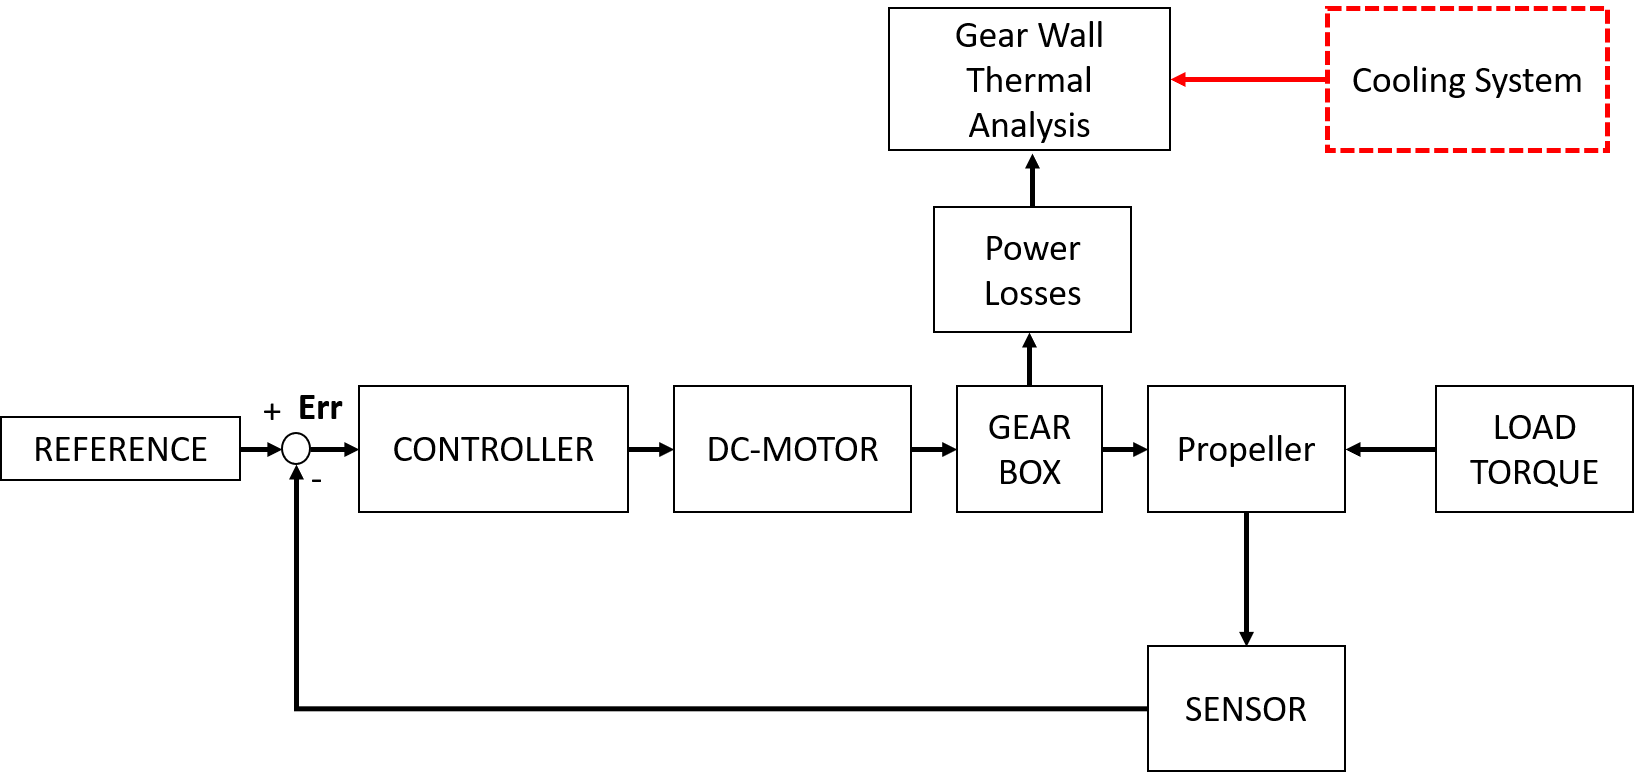
\includegraphics[width=0.9\textwidth]{gfx/BlockScheme_msas.png}
\caption{\label{fig:blocks scheme} Functional block scheme of the system.}
\end{figure}

\subsection*{2.1) Part 1: Propeller Electric Engine}
Considering the real system in \ref{fig:propeller} \textbf{without} the cooling part, you are asked to:
\begin{enumerate}
    \item Extract a physical model highlighting assumptions and simplifications.
    
    \item Reproduce the model in acausal manner in Dymola.
    
    \item According to the block scheme in \ref{fig:blocks scheme}, tune a controller (e.g., a PID controller) such that the motor input voltage remains less than 200 V and the error signal \textbf{Err} is less than 0.1 rad/s after 10 s. 

    \item Study the Gear box temperature and heat flux for a simulation time of $\mathbf{t_f}$ = 120 s (considering only conduction as heat transfer).

    \item Discuss the simulation results and the integration scheme used
\end{enumerate}

\noindent For the simulation part, you shall consider: the DC motor data listed in Table \ref{tab:dc}; the gear box data listed in Table \ref{tab:gear}, with loss parameters in Table \ref{tab:gear2}; a propeller made of \textbf{aluminium} with nominal angular speed $\hat{\omega}$ and a nominal quadratic speed load torque $\hat{T}_{load}$ acting on it (Table \ref{tab:prop}). The reference angular speed signal to be tracked by the propeller is given in Figure \ref{fig:refsignal}. 


\begin{table}[ht]
\centering
\caption{DC motor data}
\begin{tabular}{ |c|c|c| } 
\hline
\textbf{Parameter} & \textbf{Value} & \textbf{Unit}\\
\hline
Coil Resistance & 0.1 & $\Omega$  \\ 
Inductance & 0.01 & H  \\ 
Motor Inertia & 0.001 & kg $m^2$  \\ 
Motor Constant & 0.3 & Nm/A \\ 
\hline
\end{tabular}
\label{tab:dc}
\end{table}

\begin{table}[h!]
    \centering
    \caption{Gear Box data}
\begin{tabular}{ |c|c|c| } 
\hline
\textbf{Parameter} & \textbf{Value} & \textbf{Unit}\\
\hline
Mass & 3 & kg  \\ 
Gear ratio & 2 & [-]  \\ 
Specific heat & 1000 & J/(kg K)   \\ 
Thermal Conductivity & 100 & Wm/K \\ 
\hline
\end{tabular}
\label{tab:gear}
    \end{table}
    
\begin{table}[h!]
    \centering
    \caption{Gear Box Loss Table}
\begin{tabular}{ |c|c|c| } 
\hline
\textbf{Driver angular speed [rad/s]} & \textbf{Mesh efficiency[-]} & \textbf{Bearing friction torque [Nm]}\\
\hline
0 & 0.99 & 0  \\ 
50 & 0.98 & 0.5  \\ 
100 & 0.97 & 1  \\ 
210 & 0.96 & 1.5  \\ 
\hline
\end{tabular}
\label{tab:gear2}
    \end{table}

\begin{table}[h!]
    \centering
    \caption{Propeller data}
\begin{tabular}{ |c|c|c| } 
\hline
\textbf{Parameter} & \textbf{Value} & \textbf{Unit}\\
\hline
Diameter & 0.8 & m  \\ 
Thickness & 0.01 & m  \\ 
$\hat{\omega}$ & 210 & rad/s \\
$\hat{T}_{load}$ & 100 & Nm \\
\hline
\end{tabular}
\label{tab:prop}
    \end{table}



    \begin{figure}[h!]
\centering
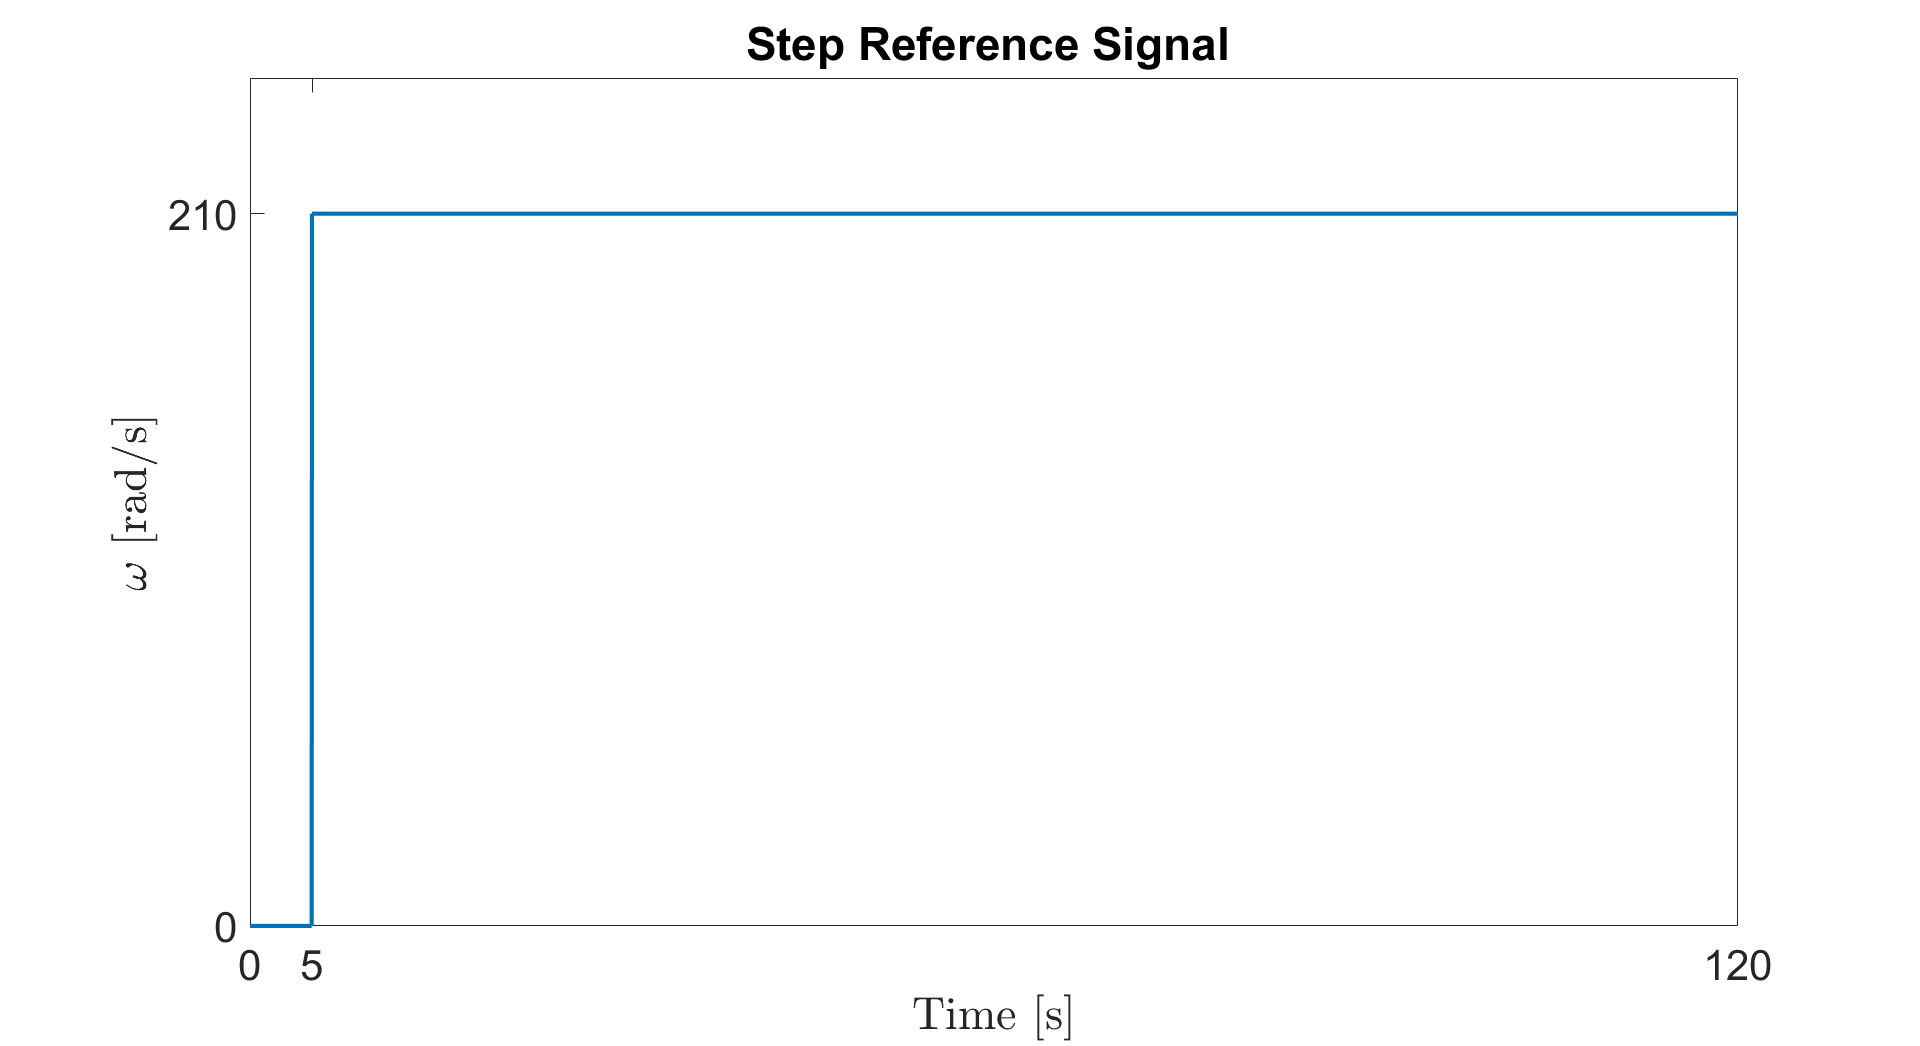
\includegraphics[width=0.8\textwidth]{gfx/ReferenceSignal.png}
\caption{\label{fig:refsignal} Angular speed reference for the propeller.}
\end{figure}



\subsection*{2.2) Part 2: Cooling System}
After the previous gear unit thermal analysis, now consider the steady-state condition reached 
by the propeller engine at the end of the simulation to model and simulate a single \textbf{fixed}
 volume flow rate cooling system (as shown in Figure \ref{fig:propeller}) for the gear unit and 
 considering only \textbf{convection} as heat transfer. In particular, you are asked to:

\begin{enumerate}
    \item Derive a physical model highlighting assumptions and simplifications.

    \item Reproduce the acausal model in Dymola.

    \item Tune the cooling system in terms of volume flow rate, control logics, and initial fluid storage temperature such that:
    \begin{enumerate}
    
        \item the gear unit is kept between 40$^{\circ}$C and 60$^{\circ}$C.
        
        \item the source tank does not get empty before the end simulation time

        \item the storage tanks have a maximum height of 0.8 $m$ and cross section area of 0.01 $m^2$
        
        \item the system shall have a recirculating capability in order to exploit the outlet fluid for a next cooling process (when the source tank get empty)
        
        \item the sink heated fluid is kept between 5$^{\circ}$C and 10$^{\circ}$C.

        \item the power consumption of the thermal system shall be no more than 6 kW 
        
    \end{enumerate}

    \item Discuss the simulation results and the integration scheme used
     
    
\end{enumerate}

\noindent For the simulation part consider properties of water at 10$^{\circ}$C as cooling incompressible fluid (convective thermal conductance $\lambda_{conv}$ = 300 W/K) and the cylindrical pipe line data listed in Table \ref{tab:pipe}. The simulation shall last at least $\mathbf{t_{sim}}$ = 300 s starting with no water along the pipe.


\begin{table}[h!]
    \centering
    \caption{Pipe line properties}
\begin{tabular}{ |c|c|c| } 
\hline
\textbf{Parameter} & \textbf{Value} & \textbf{Unit}\\
\hline
Diameter & 4 & cm  \\ 
Length & 40 & cm  \\ 
Geodetic height & 0 & m \\
Friction losses & 0 & [-] \\ 
\hline
\end{tabular}
\label{tab:pipe}
    \end{table}

    
\medskip


\medskip \hrule \medskip
\rightline{\small(15 points)}

\tr{\textit{Write your answer here}}



\clearpage

%%%%%%%%%% TO BE DELETED (BEGINS) %%%%%%%%%%
\tr{
\begin{itemize}
\item Develop \underline{one Matlab script} for Exercise 1; name the file \mcode{lastname123456_Assign2.m}. If needed, organize the script in sections and use local functions. 
\item Develop \underline{one Simulink model} for Exercise 1; name the file \mcode{lastname123456_Assign2.slx}. 
\item Develop \underline{two Dymola models} for Exercise 2; name the files \mcode{lastname123456_Assign2_Part_1.mo} and  \mcode{lastname123456_Assign2_Part_2.mo}. 
\item \underline{Create a single .zip file} containing the \underline{report in PDF}, the \underline{MATLAB file}, the \underline{Simulink model}, and the \underline{two Dymola models}. The name shall be \mcode{lastname123456_Assign2.zip}.
\item Red text indicates where answers are needed; be sure there is no red stuff in your report.
\item In your answers, \underline{be concise}: to the point.
\item \textbf{Deadline for the submission: Dec 18 2023, 23:59}.
\item \textbf{Load the compressed file to the Homework folder on Webeep}.
\end{itemize}
}
%%%%%%%%%% TO BE DELETED (ENDS) %%%%%%%%%%


\end{document}
%--------------------------------------------------------------------------------
%       END DOCUMENT
%--------------------------------------------------------------------------------